% 修論の場合は次の行を \documentclass[master]{nagasaki} とすること
\documentclass[master]{nagasaki}
\setcounter{secnumdepth}{4}
\setcounter{tocdepth}{4}
\usepackage{bm}
\usepackage[dvips]{graphicx}
\usepackage{subfigure}
\usepackage{tabularx}
\usepackage{multirow}
\usepackage{amssymb}
\usepackage{array}
\usepackage{amsfonts}
\usepackage{latexsym}
\usepackage{amsmath}
%%%%%%%%%%%%%%%%%%%%%%%%%%%
\title{論文題目}         % 論文題目
\author{野崎 大智}            % 著者
\teacher{松永 昭一 教授} % 指導教官名
\id{52117321}            % 学籍番号
\date{\today}
\date{平成29年度}        % 年度
%%%%%%%%%%%%%%%%%%%%%%%%%%%%%
\begin{document}
\maketitle
\clearpage
\pagestyle{headnombre}
\pagenumbering{roman}
\tableofcontents
\listoffigures
\listoftables
\clearpage
\pagestyle{headings}
\pagenumbering{arabic}
%%%%%%%%%%%%%%%%%%%%%%%%%%%%%
% 以下本文
\chapter{研究背景}

\section{研究背景}
近年、通信・放送業界では地上デジタル放送の開始や、新たな高速通信規格の誕生など、通信ネットワークの急速な発達が見られる。それに伴い、誰もがテレビやパソコンだけでなくスマートフォン・タブレットなど様々なデバイスを通して手軽に膨大な量の音声・映像データを入手し、好きな時に好きな場所で視聴することが容易な時代となった。そこで、映像・音声データに話者や内容のインデックスの情報が付与されていれば、必要な部分のみを容易に検索、視聴ができる。しかし、世の中には膨大な量の映像・音声データが存在するため、それら全てに人手でインデクスを付与することは事実上不可能である。そこで、自動的にインデクシングすることが望まれる。\par
自動でインデクシングを行うためには、映像・音声データ内の発話区間、発話者、発話内容の特定が必要である。これらを推定する技術のことをダイアライゼーションと呼び、本稿はこの技術の実現を目指す。\par
本稿では世の中に存在する映像・音声データの中で、ある特定の人物に情報が集中する形式で行われるニュース番組に着目した。

\vspace{0.2in}\noindent{\textbf{\underline{ニュース番組の特徴}}}
\begin{itemize}
\item 30分程度のニュース番組の中で複数の多様な話題がある
\item 1人または複数のアンカーおよび天気予報士など複数の話者が存在する
\item 話者情報(話者数、性別、話者の声質など)および発話区間が未知である
\item 対話が少ない
\item アンカーは連続で発話することが多い
\end{itemize}

\noindent このようなニュース番組において、ニュースの話題にインデクシングが行われていることは必要な話題の検索に重要である。ここで、アンカーとは司会役のアナウンサーのことであり、ニュース番組は主にアンカーを中心として進行する。アンカーの特徴は以下の通りである。

\vspace{0.2in}\noindent{\textbf{\underline{アンカーの特徴}}}
\begin{itemize}
\item 発話数が多い
\item ニュース番組の司会および話題の切り替えを行う
\item ニュース番組の全体にわたって発話している
\end{itemize}

\noindent このため、ニュース番組ではアンカーの発話に情報が集中しており、インデクシングに重要な情報を持つ。つまり、アンカーの発話区間を検出、音声認識はニュース番組のダイアライゼーションの実現に有効であると考えられる。

\section{研究目的}
特定話者の発話検出には話者特徴量(i-vector)が一般的に用いられている。また、音声認識においても認識対象の話者ごとに音声認識システムを適応させることで音声認識精度の向上が確認されている。しかし、短い発話からは話者の識別に必要なi-vectorを抽出できないことが確認されており\cite{panaiv}、アンカーの発話の誤検出、音声認識精度の低下につながる可能性がある。そこで、短い発話のi-vectorの抽出精度を向上することによって、アンカーの発話区間検出精度、音声認識精度の向上が見込めると考えた。\par
本稿では、前後の発話区間が同一話者の発話である可能性が高いとき発話区間を結合し、長い発話を擬似的に作成した。これによって短い発話のi-vectorの抽出精度向上を目指し、アンカーの発話区間検出と音声認識への有意性を検証した。検証を行なった結果、従来と比較してアンカーの発話区間検出精度が9\%、音声認識精度がhogehoge\%の向上を実現した。これにより、i-vectorの抽出において発話区間を結合し擬似的に長い発話を作成することにより、アンカーの発話区間検出、音声認識への有意性を示した。

\section{論文構成}
次章以降における本論文の構成は、まず2章で本実験で用いるシステム、アルゴリズムの概要について説明を行う。次に3章では、i-vectorの性質と評価対象であるニュース番組音声の調査を行う。4章ではi-vectorを用いたアンカーの発話検出手法と音声認識の先行研究について述べ、問題提起を行う。5章では本研究で提案するアルゴリズムの説明を行う。6章では提案手法を用いた発話区間の結合、i-vectorを再抽出を行い、アンカーの発話区間検出精度、音声認識精度への効果を検証する。7章では本研究において検証された実験の結果を元に結論を述べる。

  % 研究背景
\chapter{理論的背景}

\section{音源識別}
\section{音源分離システムの概要}
\renewcommand{\labelenumi}{(\arabic{enumi})}
音響データの中にはさまざまな音源種別(声、音楽、雑音等)の音が混在している。音源識別とは、音響データ中に含まれる音源種別を自動的に識別することである。ここでの処理は、音響データのスペクトル解析を行い、音響特徴パラメータを求め、あらかじめ用意した各音源種別の音響特徴パラメータの分布と比較することで音源種別を識別する。\par
本システムでは、ニュース番組の音声データに音響特徴パラメータを用いた音源識別\cite{shimae_9} を用い、音声データ中の音源種別を以下の4つに分類した。

\begin{enumerate}
\item 音声区間: アナウンサーやインタビューの声
\item 音楽区間: オープニングやエンディングなどの音楽、BGM
\item 背景雑音区間: 自動車走行音や鳥の泣き声、喧騒
\item 無音区間: 音量が極めて小さい区間
\end{enumerate}

また、音源識別システムは音響データを各種別へ識別するための音響特徴パラメータの分布に8混合のガウス分布を用いている。本研究の音響特徴パラメータを表\ref{table:feature_devide_audio}に示す。
\begin{table}[H]
  \begin{center}
    \caption{音源識別のための音響特徴パラメータ}
    \label{table:feature_devide_audio}
    \begin{tabular}{|c|c|} \hline
      スペクトルの変化 & スペクトルの傾き\\ \hline
      白色雑音との近さ & ピッチ  \\ \hline
      パワー & 中心周波数 \\  \hline
      中心周波数のバンド幅 &   \\ \hline
    \end{tabular}
  \end{center}
\end{table}

以降、音源識別のためのスペクトル解析と音響特徴パラメータについて説明する。\par


\subsection{スペクトル解析}
音響データのスペクトル解析の手法として最も一般的に利用されている方法は、短時間フーリエスペクトル分析がある。この方法は、音響データから連続する数10ms 程度の時間長の信号区間を切り出し、切り出された信号が定常性(一定周期で繰り返す)と仮定して、スペクトル解析を行う。\par
スペクトル解析の流れは以下の通りである。

\begin{enumerate}
\item フレーム化処理:与えられた信号$s(n)$ に長さ$N$ の窓関数を掛けることで以下のような信号系列$s_\omega(m; l)$を取り出す。
\begin{equation}
S_w(m;l)=\sum_{m=0}^{N-1}\omega(m)s(l+m)\qquad(l=0,T,2T,\cdots), \notag
\end{equation}

ここで、添え字$l$は信号の切り出し位置に対応している。すなわち、$l$を一定間隔$T$で増加させることで定常とみなされる長さ$N$の信号系列$s_\omega(n)\quad (n=0,1,\cdots,N-1)$が間隔$T$で得られる。この処理をフレーム化処理と呼び、$N$をフレーム長、$T$をフレーム間隔と呼ぶ。また、窓関数とは、ある有限区間以外で0となる関数であり、フレーム化されたデータに対して重みをつける関数である。フレーム化処理を行う場合、離散的なデータの繋ぎ目においての信号の急激な変化の影響を和らげるため、原則として窓関数をかけなければならない。代表的なものとして音声信号だけに有効なハニング窓と、音声信号以外にも様々な信号にも有効なハミング窓がある。

\begin{equation}
\label{da1}
ハニング窓:\omega(n)=0.5-0.5\cos(\frac{2\pi n}{N-1}).\qquad(n=0,1,\cdots,N-1) \notag
\end{equation}

\begin{equation}
\label{da2}
ハミング窓:\omega(n)=0.54-0.54\cos(\frac{2\pi n}{N-1}).\qquad(n=0,1,\cdots,N-1) \notag
\end{equation}

\item スペクトル分析(離散時間フーリエ変換、高速フーリエ変換):フレーム化処理によって得られた信号系列の短時間フーリエスペクトルは、離散時間フーリエ変換により以下の式で与えられる。
\begin{equation}
S(n)=\sum s_\omega(n)e^{-j2\pi \frac{nk}{N}}, \qquad (k=0,1,\cdots,N-1) \notag
\end{equation}

離散フーリエ変換(DFT) は、離散的なデータをフーリエ変換する際に、通常のフーリエ変換の無限区間積分を有限の和で書き換えたもので、時間領域、周波数領域ともに離散化されたフーリエ変換のことであり、時間領域の表現を周波数領域における表現に変換する。また、逆に周波数領域の表現を時間領域の表現に変換する、つまり元の音響データに戻す変換を離散フーリエ逆変換(IDFT) と呼び以下の式で与えられる。

\begin{equation}
S(n)=\frac{1}{N}\sum S(k)e^{j2\pi \frac{nk}{N}}. \qquad (k=0,1,\cdots,N-1) \notag
\end{equation}

実際の信号処理過程では、離散的フーリエ変換(DFT) をその高速算法である高速フーリエ変換(FFT) を用いて実行し、当該音声区間のスペクトル表現とすることが一般的である。高速フーリエ変換は式(\ref{da1}),(\ref{da2}) の$N$ が$2^n$ 個であるとき、その処理を高速にできる性質がある。フーリエ変換の式には、

\begin{equation}
S\prime(n)=S(e^{j\frac{2\pi}{n}k})=\sum s_\omega(n)e^{-j2\pi \frac{2\pi}{N}kn}, \qquad (k=0,1,\cdots,N-1) \notag
\end{equation}

なる複素系列$S\prime(k)$が音声スペクトル表現として最も一般的に用いられる。

\item パワースペクトルの算出:音響信号の離散パワースペクトル系列は、離散スペクトル系列から式(\ref{da3}) で表される。

\begin{equation}
\label{da3}
|S^\prime(k)|^2=\frac{1}{N}[\operatorname{Re}\left\{S^\prime(k)\right\}^2+\operatorname{Im}\left\{S^\prime(k)\right\}^2].
\end{equation}

この2乗値のパワースペクトル$|S^\prime(k)|^2$を特徴量として扱っている。音響信号に高速フーリエ変換を施すと、時間表現(縦軸:パワー、横軸:時間) から周波数表現(縦軸:振幅、横軸:周波数)へと変換できる。しかし、実際には縦軸を周波数、横軸を時間としたグラフがよく使用されており、このようなグラフをスペクトログラムという。スペクトログラムは音声を視覚化したものであり、声紋とも呼ばれる。

\end{enumerate}\par

\subsection{音響特徴パラメータ}
本研究で使用する7つの音響特徴パラメータについて述べる\cite{shimae_10}

\begin{enumerate}
\item スペクトルの変化\par
動的特徴量を連続するスペクトルのフレーム間の変化量として取り出す。音響信号のスペクトル分析した連続するフレームにおいて、あるフレームとその一定時間後のフレームとのパワースペクトルの差分によりスペクトルの変化量を得て、そのスペクトルの差分を一定時間足し合わせたものとしている。スペクトルの変化量によって比較する利点は、音声の識別に有利であり音声に比べて背景雑音のほうがスペクトルの変化量が大きく、無音のほうがスペクトルの変化量が小さいということである。

\item スペクトルの傾き\par
あらかじめ人手により作成したラベルにより音響データの各区間を各種別(音声、音楽、背景雑音、無音)に振り分け、それぞれに対してスペクトル分析を行い、パワースペクトルを取り出し、各種別内において集められたパワースペクトルの分布を求めることで各種別において傾き値を得る。この傾き値を基に、与えられた音響ファイルから次々に得るパワースペクトルと各種別の学習データとの特徴パラメータの分布の類似度を比較する。この最小単純形は、パワースペクトルにおける一次回帰直線の傾きを比べることと同じである。傾きによって比較する利点は、有色系の音のほうが白色雑音よりも傾きが大きいので、音声と音楽と無音の識別に有利である。

\item 白色雑音との近さ\par
パワースペクトルより一次回帰直線からスペクトル波形の切片を求めることで入力信号の白色性の度合を計測する。この白色雑音との近さによって比較する利点は、背景雑音のような定常的に混入した雑音は白色性が高いため、これらの識別ができるこということである。

\item ピッチ\par
有声音源の繰り返し周期、いわゆるピッチ(基本周波数)の変化を調べることで、音源の変化を知ることができ、音源の特定のパラメータである。周波数分析によりピッチを求め、学習データと比べることで音源の特定に用いる。

\item パワー\par
時間領域の分析だが、音響信号のような非定常的な信号に対して、変化していく信号の大きさにうまく追随するような比較的短い区間に音響データを区切り、その区間の信号$xl(n)$に対してエネルギー$E(l)$ を定義する\cite{shimae_11}。
\begin{equation}
E(l)=\sum_{n=0}^{N-1}\left\{x_l(n)\right\}^2. \notag
\end{equation}
ここでは、整数$N$ は窓の中に含まれる音響信号の数である。\par
利点としては、測定が簡単であり、音声認識における有色系の音の区間の抽出にもよく用いられることから、有音と無音の区別に有利である。

\item 中心周波数\par
抽出したパワースペクトルにおいて、無音の場合は右下がりに傾斜しているが、有音の場合は傾斜の途中で膨らみまたは突起が発生する。その突起がもっとも大きく発生している周波数帯の中心部分の周波数を中心周波数として定義している。これは有音と無音の識別に効果がある。

\item 中心周波数のバンド幅\par
中心周波数を含む膨らみ、あるいは突起の始まりと終わりによる周波数帯の長さをバンド幅として定義する。音声は一定の周波数を含むことが多いためそのバンド幅はある程度の大きさになることが考えられるが、雑音はあまり多くの周波数を含まないものから白色性が高く幅広い周波数を含むものまで様々であり、その違いから音声と雑音の特定に有効である。
\end{enumerate}\par


\section{i-vectorの概要}
近年の話者認識システムの多くは i-vector\cite{iv}に基づいて構成されおり、この領域における最高水準の技術となっている。i-vectorとは、ある発話から得られた音響特徴量を因子分析を用いて、話者固有の特徴を抽出したものである。i-vectorの抽出においては、因子分析の入力として、発話毎にGMM(Gaussian Mixture Model)の平均ベクトルを結合したGMMスーパーベクトルを用いる。発話$u$から作成された GMM スーパーベクトル$M_u∈R^{CD_F}$は以下で定義される。

\begin{equation}
M_u=T w_u + m, \notag
\end{equation}

ここで$M_u$は大量の不特定話者の発話データから作成されるUBM(Universal Background Model)を事前情報として事後確率最大化(MAP)法により推定されたGMMを用いる。
また$m$はUBMから得られる話者及びチャネル非依存のGMMスーパーベクトルである。
$C$は GMM (UBM)の混合数,$D_F$は音響パラメータの次元数、$T∈R^{CD_F*D_r}$は低ランクの矩形行列$D_r \ll CD_F$で、全変動空間を張る基底ベクトルで構成される固有声行列である。$W_u \in R^{D_r}$は発話ごとに与えられる潜在変数であり、平均ベクトルが$0 \in R^{D_T}$で共分散行列行列が単位行列$I \in R^{D_T*D_T}$のガウス分布$N(w ; 0,I)$に従う。この$w$はtotal factor(全因子)と呼ばれ、各発話に対するi-vector である。つまり、i-vectorはGMM スーパーベクトル空間における平均的な話者(UBM の平均)から「差(を次元圧縮したもの)」として各話者を表現したものと言える。

\subsection{UBMに対するBaum-Welch統計}
準備として、UBMに対するBaum-Welch統計量を計算することから始める。
$O_u={o_1,o_2,o_3,\cdots,o_L}$、$o_t\in R^{D_F}$、を発話$u$から得られる$L$フレームの音響パラメータ系列$c=1,2,3\cdots,C$、をUBM (GMM) の混合要素を表す添え字、$\Omega=\left\{\pi_c,m_c,\sum_{c}\right\}_{c=1}^{C}$をUBMのパラメータ(混合重み、平均ベクトル、対角共分散行列)とする。このとき、発話$u$に対する0次、1次、2次のBaum-Welch統計量は、

\begin{align}
N_{u,c} &=\sum_{t=1}^{L}\gamma_t(t), \notag \\
F_{u,c} &=\sum_{t=1}^{L}\gamma_t(c)(o_t-m_c), \notag \\
S_{u,c} &=diag\left[\sum_{t=1}^L\gamma_c(c)(o_c-m_c)(o_t-m_c)^\prime\right] \notag ,
\end{align}



と書ける。ここで、$y_c(c)$は、$o_t$がUBMの$c$番目の要素分布から生成される事後確率

\begin{equation}
\gamma_c(c)=\displaystyle p(c\mid o_t,Ω)=\frac{\pi_cp(o_t\mid m_c,\sum c)}{\sum_{k=1}^C \pi_kp(o_t\mid m_k,\sum k)}, \notag
\end{equation}

である。更にこれらを用いて、
\begin{align}
  N_u &= \left(
    \begin{array}{cccc}
      N_{u,1},I_{D_F} & 0 & \ldots & 0 \\
      0 & 0 & \ldots & \vdots \\
      \vdots & \vdots & \ddots & \vdots \\
      0 & 0 & \ldots & N_{u,C},I_{D_F}
    \end{array}
  \right)
\text{  $\in R^{CD_F\times CD_F}$},\\
  F_u &= \left(
    \begin{array}{cccc}
      F_{u,1} \\
      F_{u,2} \\
      \vdots\\
      F_{u,C}
    \end{array}
  \right)
\text{  $\in R^{CD_F}$},\\
  S_u &= \left(
    \begin{array}{cccc}
      S_{u,1},0 & 0 & \ldots & 0 \\
      0 & S_{u,2} & \ldots & \vdots \\
      \vdots & \vdots & \ddots & \vdots \\
      0 & 0 & \ldots & S_{u,C}
    \end{array}
  \right)
\text{  $\in R^{CD_F\times CD_F}$},
\end{align}

ここで、$I_{D_F}\in R^{D_F\times D_F}$である。

\subsection{全因子$w$の確率分布とi-vectorの抽出}
本節では、$w$に関する種々の確率分布を導出する。このとき、$w$の事後分布の導出過程においてi-vectorの具体的な計算方法を示す。

\begin{itemize}
\item 事前分布\par
$w$の事前分布は$p(w)$平均0、共分散行列を持つガウス分布であり、以下のように書ける。
\begin{equation}
\label{iv1}
p(w)\propto \exp(-\frac{1}{2}w^{\prime}w).
\end{equation}

\item 条件付き分布\par
$M_{u,c}$を混合要素に対する$M_u$の部分ベクトルとする。直感的には、$M_{u,c}$は発話$O_u$で学習したGMMの混合要素$c$に割り当てられた$O_c$の各フレームは、平均$M_{u,c}$、共分散行列$\sum_{c}$(UBMのまま)に従うと仮定する。すなわち、$w$の値で条件付けられた観測データ$O$の条件付き分布は

\begin{equation}
\label{iv2}
P(O_u|w_u)=\exp\left(\sum_{t=1}^{L}\sum_{c=1}^{C}\gamma_t(c)\log(2\pi )^{-\frac{D_F}{2}}\left|\Sigma_{c}\right|^{-\frac{1}{2}}-\frac{1}{2}\sum_{t=1}^{L}\sum_{c=1}^{C}\gamma_t(c)D(o_t;\theta_c) \right),
\end{equation}
のように書ける。ここで、

\begin{align}
D(o_t;\theta_t) &=(o_t-M_{u,c})^\prime \Sigma_{c}^{-1}(o_t-M_{u,c}), \\
M_{u,c} &=m_c+T_cw_u.
\end{align}
である。$T_c\in R^{D_F\times D_T}$は、混合要素$c$に対する$T$の部分行列である。式(\ref{iv2})のexpの内部をBaum-Welch統計量を用いて整理すると、

\begin{equation}
\begin{split}
\sum_{t=1}^{L}\sum_{c=1}^{C}\gamma_t(c)log(2\pi )^{-\frac{D_F}{2}}\left|\Sigma_{c}\right|^{-\frac{1}{2}}-\frac{1}{2}\sum_{t=1}^{L}\sum_{c=1}^{C}\gamma_t(c)D(o_t;\theta_c)=G_u^\Sigma+H_u^{\Sigma T}+\text{Const.}
\end{split}
\end{equation}

ここで、$G_u^\Sigma$及び$H_u^{\Sigma T}$は、
\begin{align}
G_u^\Sigma &=\sum_{c=1}^C\left[\frac{1}{2}N_{u,c}\log\left|\Sigma_c^{-1}\right|-\frac{1}{2}tr\left(\Sigma_c^{-1}S_{u,c}\right)\right], \\
H_u^{\Sigma T} &=w_u^\prime T^\prime \Sigma^{-1}F_u-\frac{1}{2}w_u^\prime T^\prime N_u\Sigma^{-1}Tw_u. \label{iv3}
\end{align}

\item 事後分布\par
$w$の事後分布は(\ref{iv2})〜(\ref{iv3})を用いると、

\begin{align}
%\begin{split}
p(w_u|O_u) &\propto p(O_u|w_u)p(w_u)\propto \exp(w_u^\prime T^\prime \Sigma^\prime Tw_u-\frac{1}{2}w_u^\prime w_u)\\ \notag
 &\propto exp(w_u^\prime T^\prime \Sigma^\prime F_u-\frac{1}{2}w_u^\prime N_u\Sigma^{-1}Tw_u-\frac{1}{2}w_u^\prime w_u)\\ \notag
 &\propto \exp(-\frac{1}{2}(w_u-G_uT^\prime\Sigma^{-1}F_u)^\prime G_u^{-1}(w_u-G_uT^\prime \Sigma^\prime F_u)).
%\end{split}
\end{align}
と書ける。ここで、

\begin{equation}
G_u=(I+T^\prime \Sigma^{-1}N_u T)^{-1}.
\end{equation}

である。$w$の事後分布もガウス分布であることに注意すると、平均及び分散は、

\begin{align}
\label{iv4}
E[w_u] &=G_uT^\prime \Sigma^{-1}F_u, \\
cov[w_u] &=G_u.
\end{align}

となる。前述のとおり、確率的潜在変数モデルのもと、i-vectorは$w$の事後分布の平均として得られる。つまり、発話$u$のi-vectorは、Baum-Welch統計量$N_u$、$F_u$及び推定済みのパラメータ$T$,$\Sigma$を用いて、式(\ref{iv4})により計算することができる。

\end{itemize}


\subsection{因子分析モデルパラメータの推定}
因子分析モデルのパラメータ$T$及び$\Sigma$は、EMアルゴリズムにより求められる。すなわち、完全データ${(O_u,w_u)}_{u=1}^{U}$に対する対数尤度の期待値

\begin{equation}
\label{iv5}
Q=\sum_{u=1}^{U}E[log p(O_ww_u|\theta)],
\end{equation}

の最大化問題を解くことで求める。ここで、$\theta$はパラメータ$T$、$\Sigma$を表す。完全データの対数尤度は、

\begin{equation}
\log p(O_w w_u)=logp(O_u|w_u,\theta)+logp(w_u), \notag
\end{equation}

と書けるので、式 (\ref{iv2})〜(\ref{iv3}) を用いると、式(\ref{iv5})は以下のように整理できる。

%\begin{equation}
%\label{iv6}
%\begin{split}
\begin{align}
Q=&\frac{1}{2}\sum_{u=1}^{U}\sum_{c=1}^{C}(N_{u,c} \log\left|\Sigma_c^{-1}\right|-tr(\Sigma_c^{-1}S_{u,c})), \notag  \\
&+\sum_{u=1}^{U}tr\left( \Sigma^{-1}\left( F_uE[w_u^\prime]T^\prime -\frac{1}{2}N_uTE[w_uw_u^\prime]T^\prime \right) \right) -\sum_{u=1}^{U}\frac{1}{2}tr(E[w_uW_u^\prime]). \label{iv6}
\end{align}
%\end{split}
%\end{equation}

以上より、Eステップにおいては古いパラメータを使って、$w$空間の事後分布の統計量を以下のように計算する。

\begin{align}
E[w_u] &=G_uT^\prime\Sigma^{-1}F_u, \\
E[w_uw_u^\prime] &=G_u+E[w_u]E[w_u^\prime].
\end{align}

Mステップでは、式(\ref{iv6})をパラメータに関して最大化する。まず、(\ref{iv6})を$T$に関して微分して0と置くことで、以下の関係式を得る。

\begin{equation}
\sum_{u=1}^{U}\Sigma^{-1}F_uE[w_u^\prime]=\sum_{u=1}^{U}\Sigma^{-1}N_uTE[w_uw_u^\prime].
\end{equation}

これより、$T$の推定式が、

\begin{equation}
T^i=\left(\sum_{u=1}^{U}F_u^iE[w_u^\prime] \right)\left(\sum_{u=1}^{U}N_{u,c}E[w_uw_u^\prime] \right)^{-1}.
\end{equation}

のように得られる。ここで、$T^i$、$F_u^i$は、おのおの$T$、$F_u$の$i$行目を表し、$i=(c-1)\times D_F+f$、$1\leq f\leq D_F$である。また、$\Sigma$の推定式は、

\begin{equation}
\Sigma=N^{-1}\left(\sum_{u=1}^{U}S_u-diag\left[\sum_{u=1}^{U}F_uE[w_u^\prime]T^\prime \right] \right).
\end{equation}
となる。ここで、$N=\Sigma_{u=1}^{U}N_u$である。

\subsection{コサイン類似度}
発話$x$から抽出したi-vector$w_x$と発話$y$から抽出したi-vector$w_y$の比較を行うための方法としてコサイン類似度を用いる。

\begin{equation}
\cos(w_x,w_y)=\frac{w_x\cdot w_y}{\parallel w_x\parallel\parallel w_y\parallel}.
\end{equation}

類似度の値の範囲は、$-1\leq \cos(w_x,w_y)\leq 1$であり、類似度が最も高い値は1である。



\section{i-vectorを用いたアンカーの発話区間抽出手法}
ニュース番組では、アンカー以外にインタビューイ(インタビューの受け手)や中継の有無によって話者数が大きく異なる。そのためクラスタ数を決定した場合、クラスタ数と話者数に不一致が起こり同一アンカーの発話群検出精度が低下する場合がある。そこで,同一話者の発話データのi-vectorはベクトル空間上で局所的に分布することに着目した。アンカーの発話数は非アンカーと比較して多いことから多くのアンカーの発話が局所的に集まると考えたため、同一アンカーの発話データをより精度よく検出できると考えた。\par
そこで、2つの発話データのi-vectorのコサイン類似度が閾値以上の場合、その2つの発話データの話者は同一話者であると仮定した。まず、全ての発話データ間のi-vectorのコサイン類似度を求める。次に、このコサイン類似度が閾値以上となる発話データ数が最も多い発話データを同一アンカーの発話データ群$O$のセントロイドとし、閾値以上(話者性が類似している)の全データをそのデータ群$O$の初期要素とする。\par
一方、i-vectorを抽出する発話データの発声の抑揚が大きい場合、同一話者の発話間のi-vectorであってもコサイン類似度が閾値以下になる場合がある。そこで、発話データ$u_i(\in O)$と発話データ群$O$の距離が一定距離以内であるとき、発話データ$u_i$は発話データ群$O$の要素として追加する。


\section{音声認識}
\subsection{音声認識システムの流れ}
音声認識の流れを図\ref{fig:flow_sp}に示す。まず、入力された音声データから前処理として雑音区間と無音区間を除去し、発話区間を検出する。次に検出した発話区間の音響的特徴量を抽出し、デコーダへと渡す。デコーダではこの音響的特徴量をもとに、音響モデルと言語モデル、単語辞書を参照しながら単語列の尤度を算出し、最も尤度の高いものを認識結果として出力する。言語モデルと単語辞書については\ref{language_model}節、音響モデルについては\ref{acoustic_model}節で説明する。

\begin{figure}[htb]
  \begin{center}
    \includegraphics{../../image/flow_sp.eps}
  \end{center}
  \caption{音声認識の流れ}
  \label{fig:flow_sp}
\end{figure}

\subsection{単語辞書と言語モデル}
\label{language_model}

\noindent{\textbf{\underline{単語辞書}}}\par
単語辞書には、一般的に学習データに出現する単語のなかで出現頻度の高い単語を登録する[7]。言語モデルもその単語辞書に登録された単語を用いて構築する。単語辞書の例を表\ref{table:tango}に示す。単語辞書には表記、発音形、原型、品詞番号、出現表記、音素表記などを登録する。\par

\begin{table}[htb]
  \begin{center}
    \caption{単語辞書の例}
    \begin{tabular}{|c||c|c|} \hline
      表記+発音形+原形+品詞番号 & 出力表記 & 音素表記 \\ \hline
      あか+アカ+アカ+14 & あか & a k a \\ \hline
      技術+ギジュツ+ギジュツ+1 & 技術 & g i zh j u ts u \\ \hline
      新聞+シンブン+シンブン+1 & 新聞 & sh i ng b u ng \\ \hline
    \end{tabular}
    \label{table:tango}
  \end{center}
\end{table}

音声認識では、言語モデルは、「表記+発音形+原型+品詞番号」を、音響モデルは「音素表記」の部分を用いて最尤の単語を算出する。辞書に登録している単語が少ない場合、入力された単語が辞書に登録されていないことが多くなり、他の誤った単語を出力し認識率が低下してしまう。一方、辞書に登録している単語が多すぎる場合、認識処理に時間がかかるだけでなく、認識候補が増えるため認識率が低下してしまう。よって適切な単語の登録数を検討する必要がある。

\noindent{\textbf{\underline{言語モデル}}}\par
音声認識における言語モデルとは、文の品詞や単語と単語の関係性、音素の並びの制約などを定式化したもののことである。言語モデルの主流はサンプルデータから統計的な手法によって確率推定を行なう統計的言語モデルである。その中でも最も広く使われているのが$N$グラムモデルである。\par
\noindent{\textbf{\underline{$N$グラムモデル}}}\par
$N$グラムモデルとは、与えられた単語列$\omega_1,\omega_2,\cdots,\omega_n$に対して、その出現確率$p(\omega_1,\omega_2,\cdots,\omega_n)$を推定する場合に、

\begin{equation}
P(\omega_1,\omega_2,\cdots,\omega_n)=\prod_{i=1}^{n}p(\omega_{i}\mid \omega_{i-N+1}\cdots \omega_{i-1})
\end{equation}

のような近似を行なうモデルである。$N$グラムモデルでは、$i$番目の単語$ω_i$の生成確率が、直前の$N-1$単語$ω_{i-N+1}\cdots ω_{i-2}ω_{i-1}$だけに依存すると考える。特に$N = 1$のときユニグラム(unigram)、$N = 2$のときバイグラム(bigram)、$N = 3$のときトライグラム(trigram)という。\par
文や発話中の単語の生成確率は文脈に依存することから、$N$グラムモデルの推定確率は、$N$が大きいほど高くなる。しかし、$N$グラムモデルは語彙の$N$乗のコストがかかることから、$N$を大きくするためには、膨大な量のテキストを用意しなければならない。しかし、自由発話を記述したテキストは極めて少ない。本研究では、$N = 3$のtrigramを用いる。\par



\subsection{音響モデル}
\label{acoustic_model}
音響モデルとは、音声の最小単位である音素または、単語や音節の音響特徴パラメータの時系列をモデル化したものである。この音素の特徴は、発話者や発話内容などによって変化するが、発話者ごと、または発話タスクごとにモデル化することは、膨大なコストがかかり汎用性がないため好ましくない。そのため、音響モデルの構築方法としては、音素ごとに様々な学習音声で学習を繰り返し、最尤の音響モデルを作ることが一般的である。本研究では、隠れマルコフモデル(Hidden Markov Model)を用いて最尤の音響モデルを構築する。\par
以下に音響モデルを構築する際に、必要となる知識について述べる。\par


\noindent{\textbf{\underline{MFCC}}}\par
メル周波数ケプストラム係数(Mel - Frequency Cepstrum Coefficient : MFCC)とは、メル周波数という人間の音の高低に対する感覚尺度で音声スペクトルから係数スペクトルを抽出したものである[7]。これは一般的に、音声の特徴を抽出するパラメータとして用いられる。
 MFCCの計算では、スペクトル分析は周波数軸上に$L$個の三角窓を配置し、フィルタバンク分析により行なう。すなわち、窓の幅に対応する周波数帯域の信号のパワーを、単一スペクトルチャネルの振幅スペクトル $|S^\prime (k)|$ の重み付けの和$m(l)$ で求める。

\begin{equation}
m(l)=\sum_{k=lo}^{hi}W(k;l)\mid S^\prime(k)\mid \quad (l=1,\cdots,L)
\end{equation}

\begin{equation}
W(k;l)=\begin{cases}\frac{k-k_{lo}(l)}{k_c(l)-k_{lo}(l)}\quad \{k_{lo}\leq k \leq k_c(l)\} \\\frac{k_hi(l)-k}{k_{hi}(l)-k_{l}(l)}\quad \{k_{c}\leq k \leq k_{hi}(l)\} \end{cases}
\end{equation}

ただし、$W(k;l)$ は重み、$k_{lo}(l)、k_c(l)、k_{hi}(l)$ はそれぞれ$l$番目のフィルタの下限、中心、上限のスペクトルチャネル番号であり、隣り合うフィルタ間で

\begin{equation}
k_c=k_{hi}(l-1)=k_{lo}(l+1)
\end{equation}

なる関係がある。さらに、$k_c(l)$はメル周波数軸上で等間隔に配置される。メル周波数は

\begin{equation}
Mel(f)=2595\log_{10}(1+\frac{f}{700})
\end{equation}

により計算される。ただし、$f$の単位は[Hz]にとる。\par
最終的にフィルタバンク分析により得られた$L$個の帯域におけるパワースペクトルを離散コサイン変換することで、式(\ref{eq:mfcc})のようにMFCCが得られる。

\begin{equation}
\label{eq:mfcc}
c_{mfcc}(i)=\sqrt{\frac{2}{N}}\sum_{i=1}^{L}\log ml \cos \left\{ \left( l-\frac{1}{2}\frac{i\pi}{L} \right)\right\}
\end{equation}


\noindent{{\textbf{\underline{隠れマルコフモデル(HMM)}}}\par
\noindent{{\textbf{\underline{調音結合}}}\par

\subsection{DNNの概要}

   % 基礎理論
\chapter{提案手法}

ていあんしゅほう

\begin{figure}[htb]
  \begin{center}
    \includegraphics{./figure/piano.eps}
  \end{center}
  \caption{ぴあの}
  \label{fig:one}
\end{figure}


\begin{figure}[htb]
  \begin{center}
    \includegraphics{./figure/piano.eps}
  \end{center}
  \caption{ぴあの}
  \label{fig:one}
\end{figure}

 % 提案手法
\chapter{評価実験}

ひょうかじっけん

\section{予備実験}
\subsection{実験目的}
しきいちきめるよー

\subsection{実験条件}
おおざっぱだよー


\section{本実験}
\subsection{実験目的}
ひょうかするよー

\subsection{実験条件}
よびといっしょだよー

\begin{table}[htb]
  \begin{center}
    \caption{実験結果}
    \begin{tabular}{|c||c|c|c|} \hline
      被験者 & 実験1 & 実験2 & 実験3 \\ \hline
      AAA & 3 & 5 & 3 \\ \hline
      BBB & 1 & 2 & 4\\ \hline
      CCC & 5 & 5 & 6 \\ \hline
      DDD & 5 & 0 & 8\\ \hline
    \end{tabular}
  \end{center}
\end{table}


\section{考察}
こうさつするよー

    % 評価実験
\chapter{結論}

けつろん
  % 結論
\chapter{追加}

追加
  % 追加してみた
\chapter*{謝辞}

最後に,本研究および本修士論文作成にあたり暖かい御指導および適切な御助言をして頂いた松永 昭一教授,高田 寛之助教,山下 優博士に心より感謝いたします.

また,同研究室
博士前期(修士)課程2年の三浦 亮氏,
博士前期(修士)課程1年の入口 佳佑氏,堤 彬人氏,福永 慶士氏,
学士課程4年の平野 吉則氏,Zhang Tianzhi氏,
阿利 迪洋氏,梅野 直幹氏,古賀 光氏,増田 紗依氏,松本 優里奈氏,その他関係各位に心から感謝いたします.
    % 謝辞
\addcontentsline{toc}{chapter}{謝辞}
\begin{thebibliography}{99}     %文献数が10未満の時 {9}
\bibitem{yamaguchi_indexing}山口 正秀,松永昭一,山下優,"Spectral Cross-Correlation Features for Audio Indexing of Broadcast News and Meetings",Eurospeech,pp613-615(2005)
\bibitem{yoshimura_clustering}吉村竜哉,"話者クラスタ音響モデルを用いた会議音声認識のための話者適応",電気情報通信学会九州支部学生会講演会(2014)
\bibitem{iv}N.Dehak, P.Kenny, R.Dehak, P.Dumouchel and P.Ouellet,"Front-end factoranalysis forspeaker verifiCatiOn" IEEE Trans. Audio Speech Lang. Process, 19, 788-798(2011)
\bibitem{nozaki_gakuseikai}野崎大智,"ニュース音声におけるi-vectorを用いた同一アンカーの発話群の検出",電気情報通信学会九州支部学生会講演会(2018)
\bibitem{adachi_gakuseikai}安達大輔,"ニュース番組における発話者群の段階的分類の検討",電気情報通信学会九州支部学生会講演会(2012)
\bibitem{panaiv}辻川美沙貴,西川剛樹,松井知子,"i-vectorによる短い発話の話者識別の検討",電子情報通信学会(2015)
\bibitem{ATR}国立情報学研究所データセット集合利用研究開発センター"ATRバランス文"
\bibitem{alize}"ALIZE",http:/alize.univ-avignon.fr
\bibitem{shimae_9}冨久祐介,“音源識別のための音クラスタリングとガウス分布混合数の有効性の検討”,
長崎大学工学部情報システム工学科平成,19年度卒業論文(2008)
\bibitem{shimae_10}水野理, 大附克年, 松永昭一, 林良彦: “ニュースコンテンツにおける音響信号自動判
別の検討”, 電気情報通信学会総合大会(2003)
\bibitem{sp_recognition_shikano}:鹿野清宏,伊藤克亘,河原達也,武田一哉,山本幹雄,"音声認識システム",情報処理学会,オーム社(2003)
\bibitem{audio_textbook}河原達也,"音声認識システム",情報処理学会(2016)
\bibitem{kaldi}"KALDI",http://kaldi.sourceforge.net/
\bibitem{kojima}小島和也,"会議音声認識のためのDNNを用いた高精度な音響モデルの構築法の検討",長崎大学工学部情報システム工学科 平成25年度修士論文(2013)
\bibitem{egashira_text}江頭一茂,"会議の発話分の特徴に合わせた会議音声認識用言語モデルの構築法の検討",長崎大学工学部情報システム工学科,平成25年修士論文(2013)
\bibitem{arai_text}荒井勇吏,"会議音声認識のための発話行為依存言語モデルの構築",長崎大学工学部情報システム工学科,平成26年修士論文(2014)
\bibitem{shimae_11}新美康永,“音声認識”,共立出版株式会社(1979)
\end{thebibliography}
    % 参考文献
\addcontentsline{toc}{chapter}{参考文献} 

% 付録がある場合
%\appendix
%\input{app}    % 付録

\end{document}
